\documentclass{minimal}

\usepackage{amssymb}
\usepackage{mathtools}
\usepackage{algorithm}
\usepackage{algpseudocode}

\usepackage{tikz}


\begin{document}
	
\begin{tabular}{ p{4cm} p{0.5cm} l }
	\(\mathbf{C}\) &:& Cities \\
	\({D_{m,n}} \in \mathbf{D}\ \forall\ m,n \in \mathbf{C}\) &:& Distance Matrix \\
	\({T_{m,n}} \in \mathbf{T}\ \forall\ m,n \in \mathbf{C}\) &:& Tinder Matrix \\
\end{tabular}

\vspace{4em}


\begin{algorithm}
\caption{Forest Fire}
\label{alg:forest_fire}
\begin{algorithmic}
%\color{lightgray}

	\Procedure{}{Iterations, $\mathbf{D}$, $\mathbf{T}$, burn rate, growth rate}
	
	\(r^\prime = \) an empty list with length = the number of cities 

	\(d^\prime = \) some very large number

	\For{i in Iterations}
	
		Initialize arrays to store visited cities \(\mathbf{C}_V\) and unvisited cities \(\mathbf{C}_U\)
		
		Choose a random city, \(m \ \in \mathbf{C}\)
		
		\(r \gets m\)

		\(\mathbf{C}_V\) \(\overset{m}{\leftarrow}\) \(\mathbf{C}_U\)
		
		\While{un-visited cities \(> 0\)}
			\State \(\mathbf P\gets  D_{m,n}^{-T_{m,n}}, \quad\forall n \in\mathbf{C}_U\)
			%\Comment{Calculate city visit probabilities} 
			%(More Tinder > higher probability)
			
			\State Normalize \(\mathbf{P}\)
			
			\State Choose the next city \(n\) using \( \mathbb P(X=n) = \mathbf{P}_n \)

			\State \(T_{m,n} \gets T_{m,n} - \) burn rate
			
			\State \(\mathbf{T} \gets \mathbf{T} + \) growth rate \(\times \exp[D_{m,n}]\)
			
			\State \(m \gets n\)
			
			\State \(\mathbf{C}_V\) \(\overset{m}{\leftarrow}\) \(\mathbf{C}_U\)
			
			\State \(r \gets m\)
		\EndWhile
		
\color{black}

		\State Route Length \(\gets \sum_{}^{j\in r} D_{j,j+1} \)
		
		\If{Route Length $<$ Best Route Length}
			\State \(r^\prime \gets r\)
		\EndIf
		
		\Return \(r^\prime\) and Best Route Length

	\EndFor
	\EndProcedure

\color{lightgray}		
		
\end{algorithmic}
\end{algorithm}


\hspace{5em}


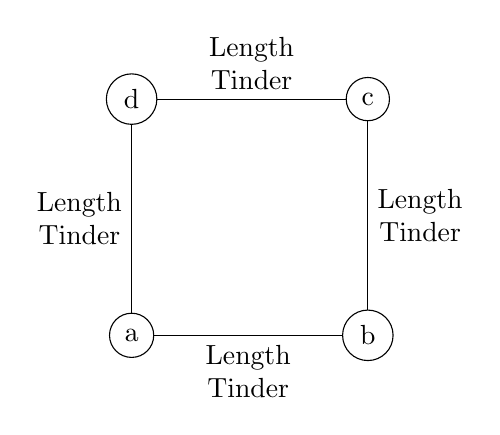
\begin{tikzpicture}
	% Define nodes
	\node [circle, draw] (a) at (0,0) {a};
	\node [circle, draw] (b) at (3,0) {b};
	\node [circle, draw] (c) at (3,3) {c};
	\node [circle, draw] (d) at (0,3) {d};
	
	% Draw edges and label them
	\draw (a) -- node[midway, below, align=center] {Length \\ Tinder} (b);
	\draw (b) -- node[midway, right, align=center] {Length \\ Tinder} (c);
	\draw (c) -- node[midway, above, align=center] {Length \\ Tinder} (d);
	\draw (d) -- node[midway, left, align=center]  {Length \\ Tinder} (a);
\end{tikzpicture}










\end{document}